\chapter{Gaussian Naive Bayes} \label{chp:bayes}
La precedente fase di analisi ha permesso di acquisire informazioni utili sulla
struttura del dataset e di conseguenza permettere la selezione di un modello
adatto a svolgere il compito di classificazione.

In questo capitolo verranno presentati tutti i risultati ottenuti dall'apprendimento
e dalle valutazioni effettuate sul modello Gaussian Naive Bayes. Da notare che 
si sta utilizzando Gaussian Naive Bayes pur sapendo che non tutte le features 
derivano da una distribuzione normale, siamo consci del fatto che non si stanno 
rispettando le assunzioni del modello.

\section{Addestramento di Gaussian Naive Bayes}
Sono stati creati due modelli allenati rispettivamente sul training set di Dateset-corr
e Dateset-pca. In aggiunta, non è stato effettuato nessuno studio degli iperparametri
dal momento Gaussian Naive Bayes non possiede degli iperparametri che devono essere
stimati.

\section{Risultati}

Dati i due modelli addestrati precedentemente, sono state effettuate le previsioni
sui test set dei rispettivi dataset utilizzati nell'apprendimento e, infine,
sono state calcolate le metriche di valutazione.

Per prima cosa è stata calcolata la matrice di confusione per ciascun modello,
visibile nella figura \ref{fig:matrice_di_confusione_per_GNB}.

\begin{figure}[!ht]
    \centering
    \begin{subfigure}{0.45\textwidth}
        \centering
        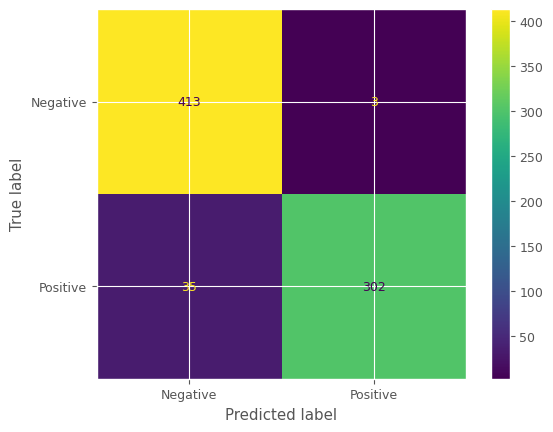
\includegraphics[width=\textwidth]{img/gnb/confusion_matrix_corr.png}
        \caption{Gaussian Naive Bayes allenato su Dataset-corr}
        \label{fig:matrice_di_confusione_per_GNB_corr}
    \end{subfigure}
    \hfill
    \begin{subfigure}{.45\textwidth}
        \centering
        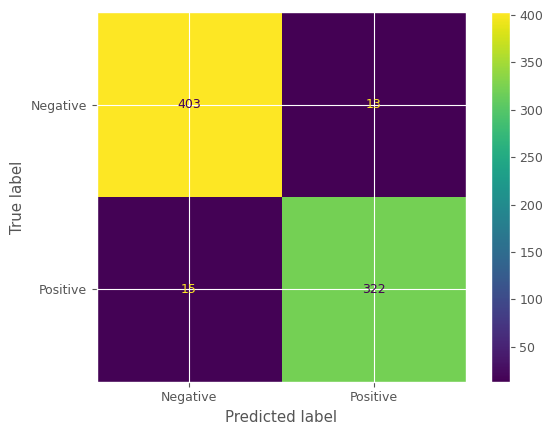
\includegraphics[width=\textwidth]{img/gnb/confusion_matrix_pca.png}
        \caption{Gaussian Naive Bayes allenato su Dataset-pca}
        \label{fig:matrice_di_confusione_per_GNB_pca}
    \end{subfigure}
    \caption{matrici di confusione per Gaussian Naive Bayes}
    \label{fig:matrice_di_confusione_per_GNB}
\end{figure}

Le matrici di confusione evidenziano come i modelli generalizzano molto bene, più
precisamente il modello allenato su Dataset-corr ha un'accuracy del $95\%$, al contrario
quello allenato su Dataset-pca raggiunge un'accuracy del $96\%$. Questo denota che 
ridurre le dimensioni del dataset utilizzando pca non porta a significativi miglioramenti
sulle predizioni. Questo mancato miglioramento può essere dovuto al fatto che si
è già trovata una buona ipotesi vicina alla funzione generatrice del dataset.

Dalle matrici di confusione oltre all'accuracy si possono calcolare le metriche
di precision, recall e F1-score, i loro valori sono visionabili nella tabella 
\ref{tab:risultatiBayes}.

\begin{table}[!ht]
    \centering
        
    \begin{tabular}{|c|c|c|}
        \hline
        \textbf{Metrica} & \textbf{Valore sul training set di Dataset-corr} & \textbf{Valore sul training set di Dataset-pca} \\
        \hline
        Accuracy & $95\%$ & $96\%$ \\
        \hline
        Precision & $90\%$ & $96\%$ \\
        \hline
        Recall & $99\%$ & $96\%$ \\
        \hline
        F1 score & $94\%$ & $96\%$ \\
        \hline
    \end{tabular}
    \caption{Metriche Gaussian Naive Bayes}
    \label{tab:risultatiBayes}
\end{table}

Dalle metriche di valutazione si può notare come su Dataset-corr si ha una precision
minore rispetto alla recall, quindi significa che si tende ad associare la presenza
di un tumore anche quando non è presente. Al contrario su Dataset-pca aumenta la
precision diminuendo la recall, questo significa che sarà più affidabile su un 
riscontro positivo rispetto ad un riscontro negativo.